\chapter{Opis projektnog zadatka}

Cilj ovog projekta je razviti programsku potporu za stvaranje web aplikacije \textit{"SkillEtCooking"} koja će korisniku olakšati snalaženje u kuhinji i optimizaciju iskorištavanja sastojaka koje osoba već posjeduje. Na taj način korisnik neće morati provesti cijeli dan razmišljajući što i kako napraviti nego to aplikacija radi umjesto njega.
\newline Sustav će podržavati više vrsta korisnika:
\begin{packed_item}
	\item registrirani
	\item neregistrirani
	\item moderatori.
\end{packed_item}

Neregistriranim korisnicima se prilikom otvaranja aplikacije otvori početna stranica na kojoj se nalaze svi recepti (\ref{fig:promjene}). Recepti se mogu sortirati na razne načine:

\begin{packed_item}
	\item popularnost
	\item prosječna ocjena recepta
	\item oznaka "Preporučeno".
\end{packed_item}

Popularnost se određuje na osnovu broja otvaranja pojedinog recepta dok se sortiranje po oznaci "Preporučeno" određuje na osnovu prosjeka popularnosti i prosječne ocjene koristeći funkciju:

\begin{packed_item}
	\item ocjena/prosjecnaOcjena + brojOtvaranja/prosjecniBrojOtvaranja
\end{packed_item}

\begin{figure}[H]
	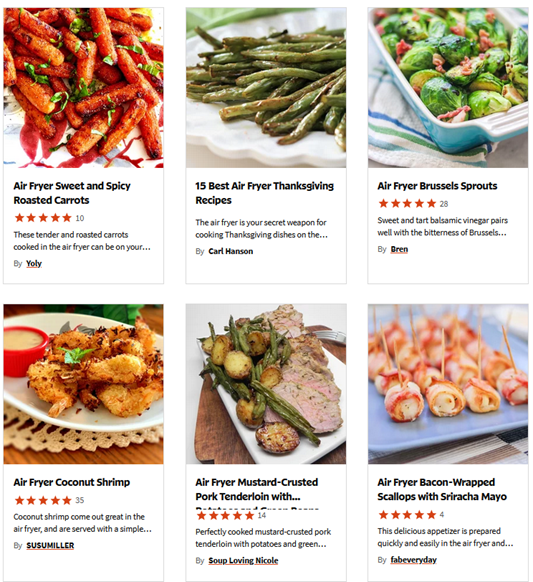
\includegraphics[scale=0.8]{slike/Slika1.PNG} %veličina slike u odnosu na originalnu datoteku i pozicija slike
	\centering
	\caption{Prikaz svih recepata}
	\label{fig:promjene}
\end{figure}
Neregistrirani korisnici imaju mogućnost filtriranja recepata upisivanjem imena recepta ili sastojka/sastojaka. Nakon filtriranja skupa recepata po sastojcima, recepti se sortiraju po vrijednosti Jaccardovog indeksa sličnosti s time da najsličniji dolazi prvi te se izbacuju svi recepti čija je vrijednost indeksa sličnosti manja od praga. Za to vrijeme, ostali izbori sortiranja su onemogućeni, ali pretraživanje po naslovu je i dalje u funkciji.

Sljedeća mogućnost neregistriranih korisnika je da im se pritiskom na naziv recepta prikazuje stranica s detaljima recepta. Na toj stranici vidljivi su svi podatci vezani za recept:

\begin{packed_item}
	\item slika
	\item naziv
	\item procijenjeno vrijeme kuhanja
	\item sastojci i količina svakog sastojka
	\item koraci pripreme s kratkim opisom
	\item ocjena (\ref{fig:promjene2}).
\end{packed_item}

\begin{figure}[H]
	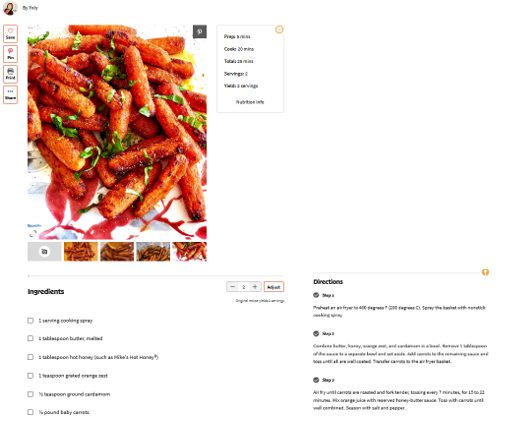
\includegraphics[scale=0.8]{slike/Slika2.PNG} %veličina slike u odnosu na originalnu datoteku i pozicija slike
	\centering
	\caption{Primjer otvorenog recepta}
	\label{fig:promjene2}
\end{figure}

Stranica sadrži prostor sa komentarima i ocjenama gdje je moguće vidjeti iskustva drugih korisnika što će biti izvedeno korištenjem Disqus usluge (\ref{fig:promjene3}). Tu je vidljiva prva razlika između registriranog i neregistriranog korisnika, a to je da komentare i ocjene mogu ostaviti samo registrirani korisnici. Također ukoliko je autor ostavio komentar na svoj recept, komentar će biti dodatno naglašen i bolje uočljiv ostalim korisnicima.

Osim toga, stranica sadrži i mogućnost da klikom na gumb korisnik može pregledati sve ostale recepte s istim autorom kao i odabrani recept.

Registrirani korisnik se može prijaviti, a neregistrirani će imati mogućnost registracije u sustav (\ref{fig:promjene4}). Prijavljeni korisnik može koristiti aplikaciju na jednak način kao i neprijavljeni korisnik, ali prijavljeni korisnik također može dodavati i uređivati vlastite recepate, uređivati vlastite podatke te koristiti prethodno objašnjenu funkcionalnost ostavljanja komentara. Pravila prilikom unosa recepta su da korisnik mora unijeti sliku jela (maksimalno 5), barem jedan sastojak i količinu te barem jedan korak pripreme.
\begin{figure}[H]
	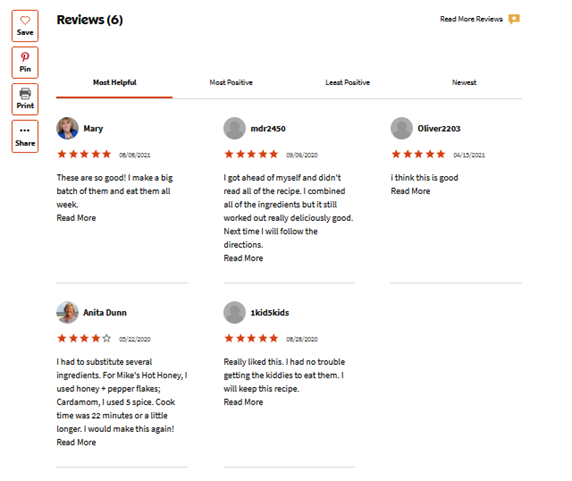
\includegraphics[scale=0.8]{slike/Slika3.PNG} %veličina slike u odnosu na originalnu datoteku i pozicija slike
	\centering
	\caption{Komentari na recept}
	\label{fig:promjene3}
\end{figure}

\begin{figure}[H]
	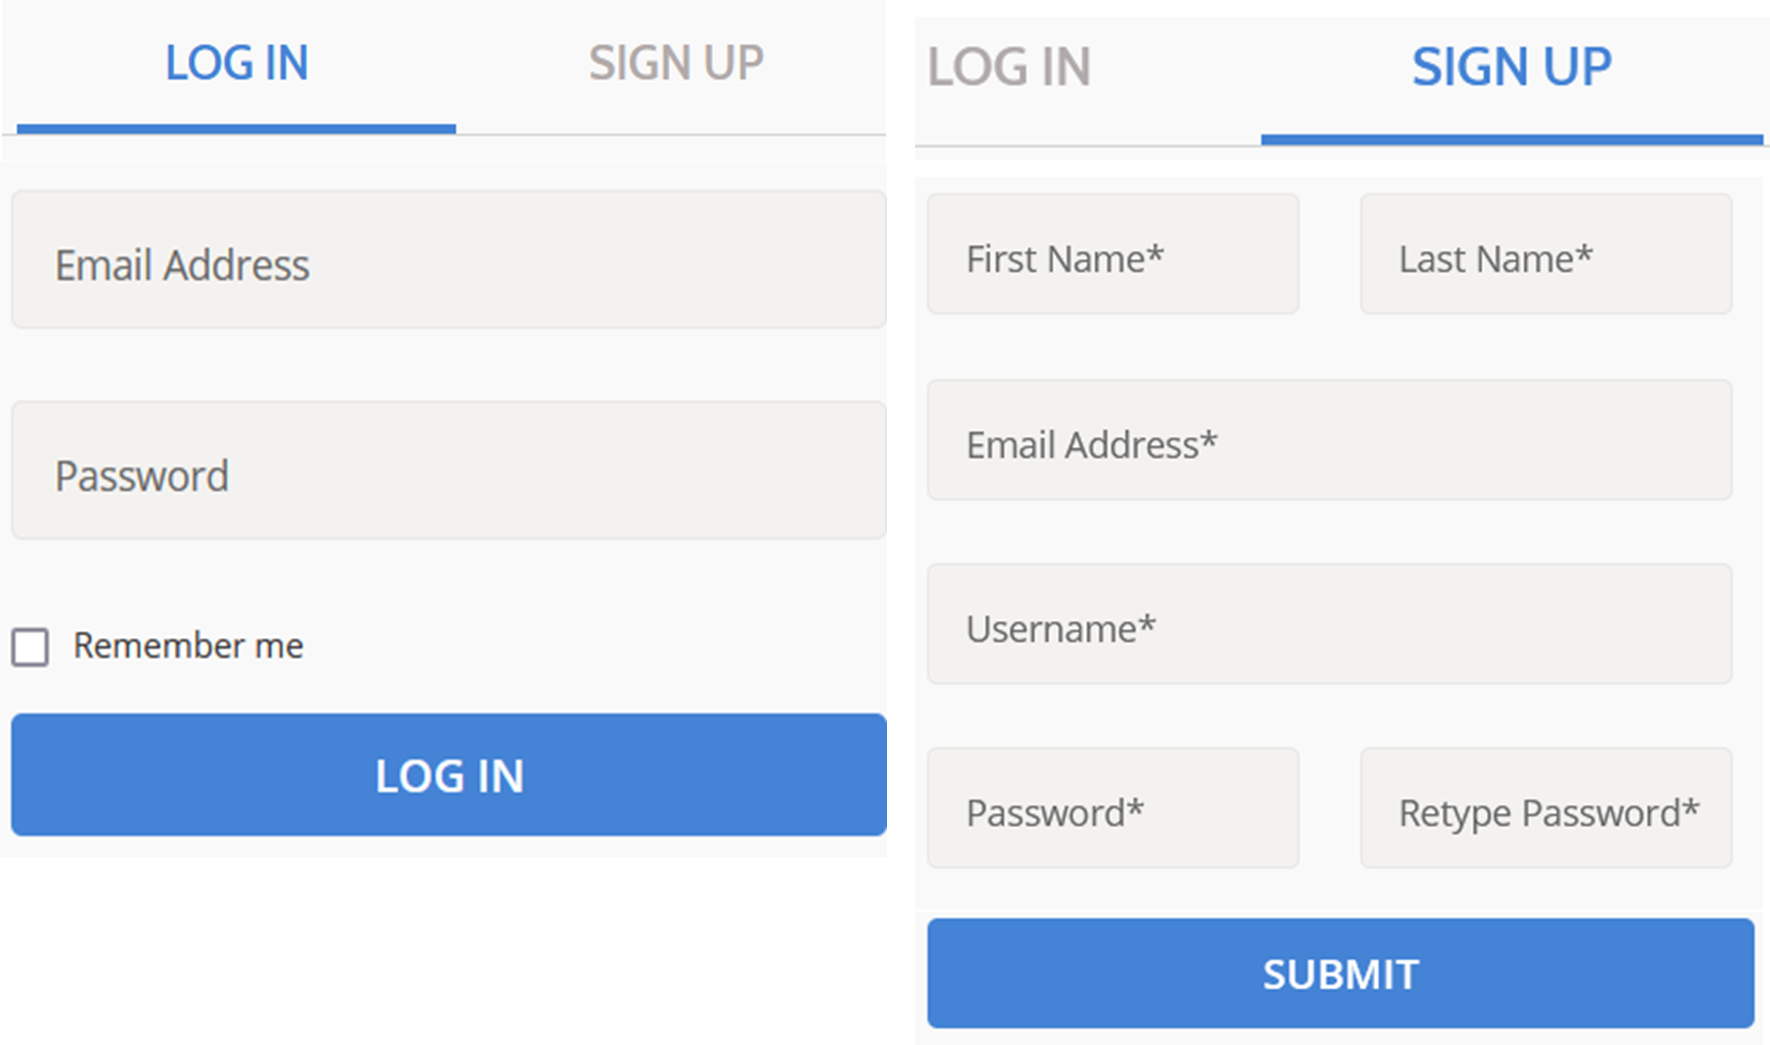
\includegraphics[scale=0.8]{slike/Slika4.PNG} %veličina slike u odnosu na originalnu datoteku i pozicija slike
	\centering
	\caption{Prijava i registracija u sustav}
	\label{fig:promjene4}
\end{figure}

Sustav koriste i moderatori koji su interni zaposlenici projekta, a njihovi računi se dodaju direktno u bazu podataka. Moderatori se prijavljuju u sustav jednako kao i ostali korisnici. Oni mogu dodati komentar na nekome receptu koji će kao i kod autora  biti dodatno vizualno označen, ali ne mogu ocjenjivati recepte.
\newline

Dodatne mogućnosti moderatora su:

\begin{packed_item}
	\item brisanje komentara
	\item brisanje recepata
	\item pregled korisnika sustava.
\end{packed_item}
Također sustav mora biti funkcionalan ukoliko je više korisnika prijavljeno u isto vrijeme neovisno o tome jesu li moderatori ili obični registrirani korisnici.


\eject



